%%____________________________________________________________________________||
\section{Study on the most sensitivity categories per each model}
\label{sec:sensitivity-study}
As mentioned in Section \ref{sec:susy}, the signal extraction is performed with a likelihood fit including the 
10 most sensitive $(\njet,\nb)$ categories. 
The following procedure is applied for each benchmark model separately.

\begin{itemize}
\item The datacards for each $(\njet,\nb,\HT)$ bin are created separately
\item The \HT bins within the same $(\njet,\nb)$ category are combined
\item Exclusion limit and discovery significance are computed for each $(\njet,\nb)$ category
\item $(\njet,\nb)$ categories are ranked according either to largest significance or smaller exclusion limit
\item The first 10 $(\njet,\nb)$ categories from the ranked list are combined to produce the final result
\end{itemize}

Both figures of merit, exclusion and discovery, have been tested and checked to give almost identical results. 
For all the benchmark models, in fact, the categories driving the sensitivity are usually few, 
and the two different approaches always agree in identifying at least the first ~5 categories. 
For the results presented in this note, the exclusion limit has been used, but we foresee to switch soon 
to use the significance as a figure of merit. 
We do not expect the conclusions of this study to be significantly
affected by the use of the exclusion limit (as opposed to
significance) as the figure of merit for the benchmark models
considered.

In Figure \ref{fig:muVsCat} the exclusion limit is presented as a function of the number of categories 
included in the fit, after the ranking procedure described above, for all the benchmark models. 
The absolute value of the exclusion limit in Figure \ref{fig:muVsCat} cannot be directly compared with the numbers reported in Table \ref{tab:results_ul}, 
because the study presented here was carried on with a different
integrated luminosity scenario and does not include the latest
development in the signal extraction strategy 
(\ie the use of \mht templates taken from simulation). Again, we do
not expect the conclusions of this study to be significantly affected
by this recent change, for the benchmark models considered. 
It may be noticed that the metric of 10 categories catches almost 100\% of the full sensitivity 
for all the models investigated so far.

\begin{figure}
  \begin{center}
    \subfigure[{\scriptsize SMS\_T1bbbb\_2J\_mGl1000\_mLSP900}]{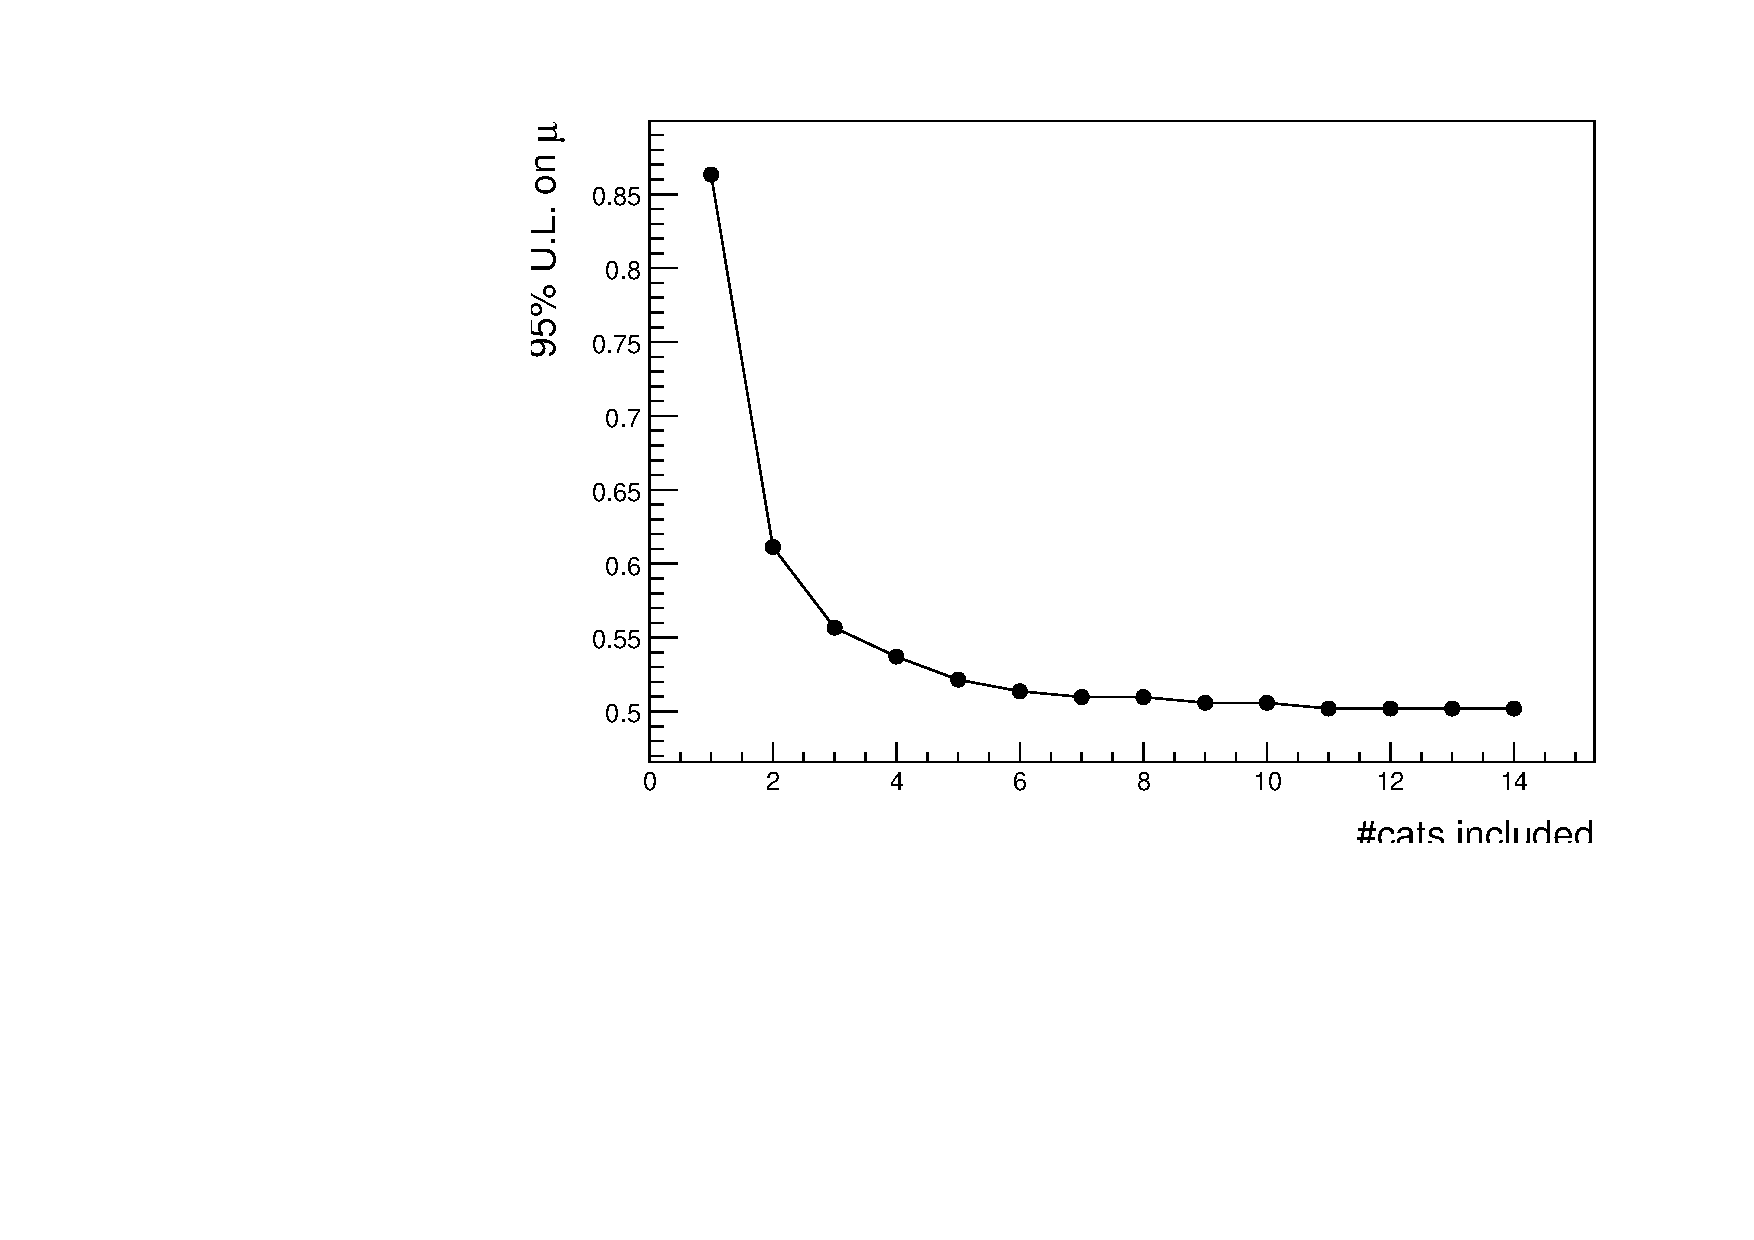
\includegraphics[width=0.31\textwidth]{figures/sensitivityStudy/MuVsCat_SMS_T1bbbb_2J_mGl1000_mLSP900.pdf}} ~~
    \subfigure[{\scriptsize SMS\_T1bbbb\_2J\_mGl1500\_mLSP100}]{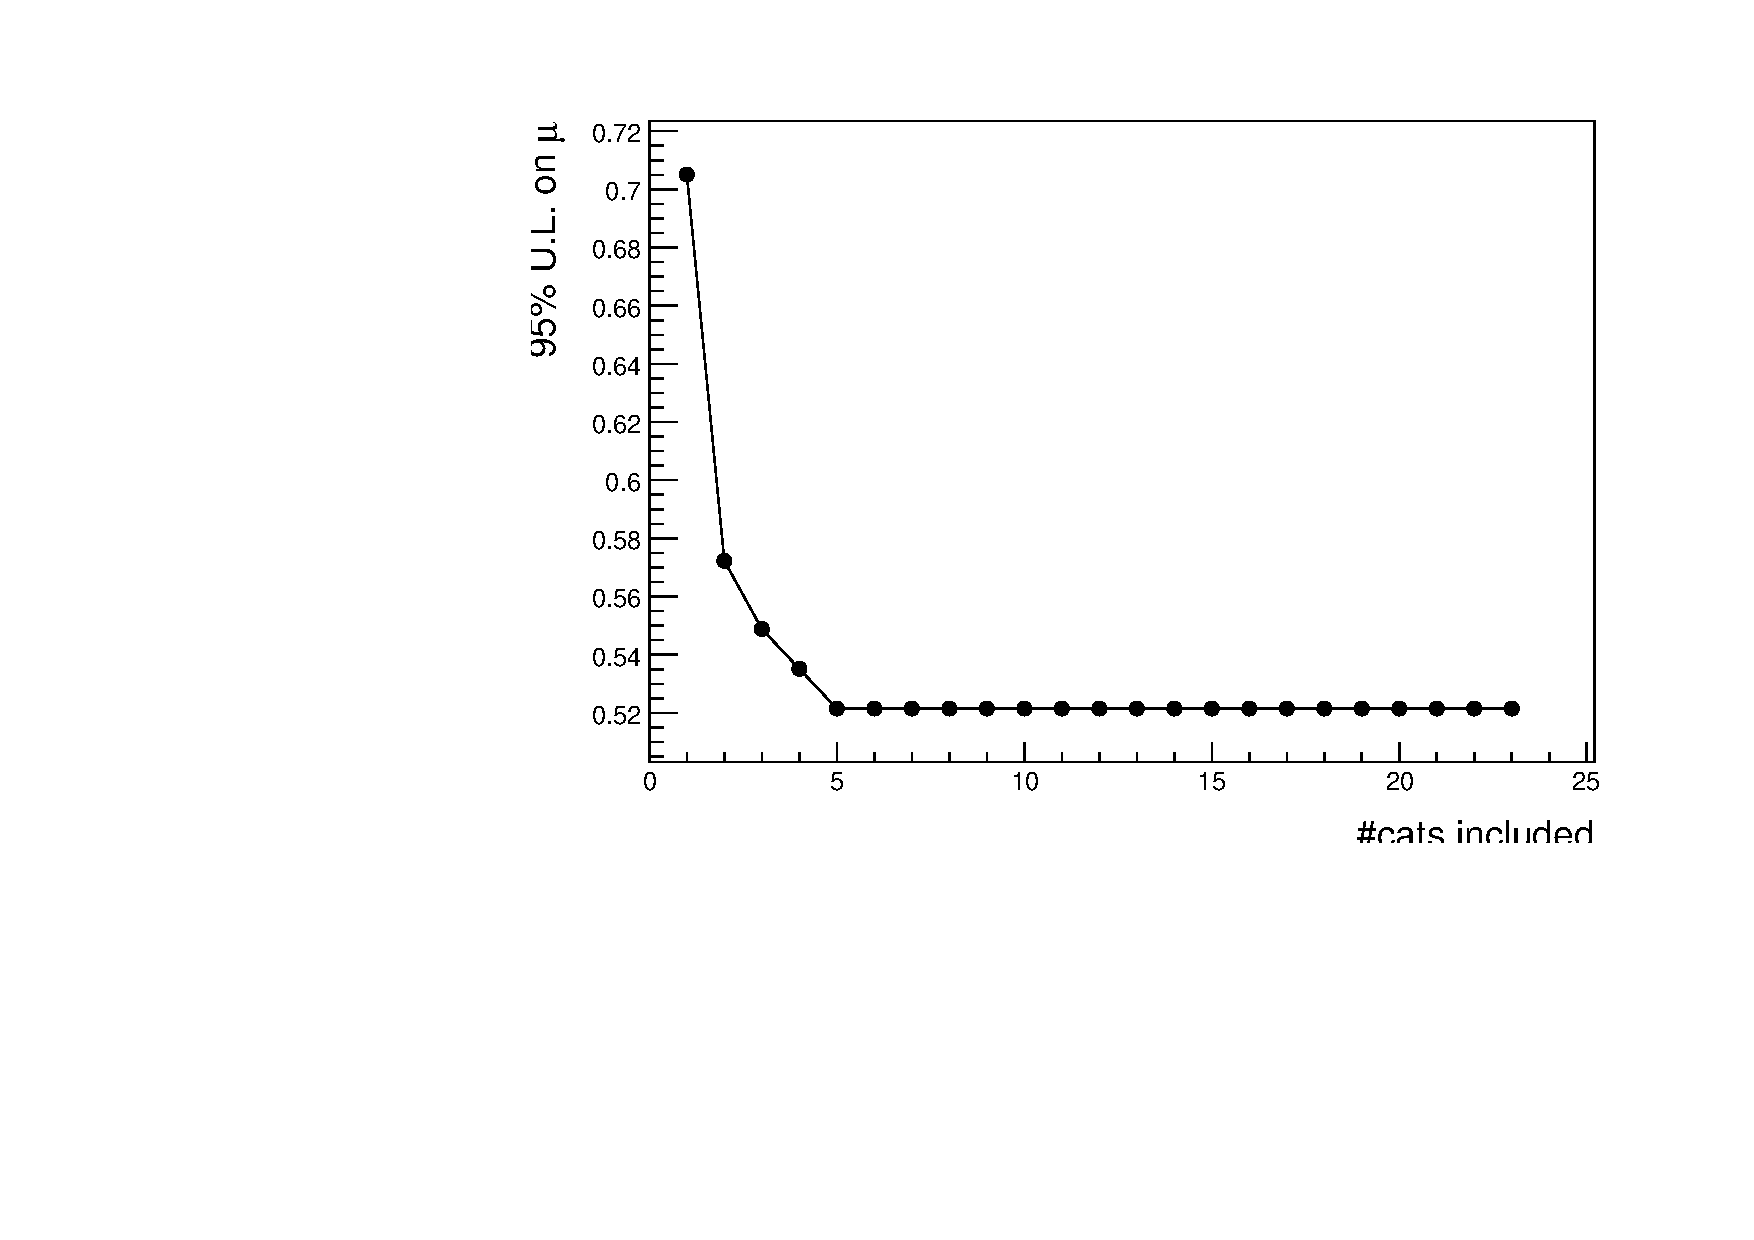
\includegraphics[width=0.31\textwidth]{figures/sensitivityStudy/MuVsCat_SMS_T1bbbb_2J_mGl1500_mLSP100.pdf}} ~~
    \subfigure[{\scriptsize SMS\_T1qqqq\_2J\_mGl1000\_mLSP800}]{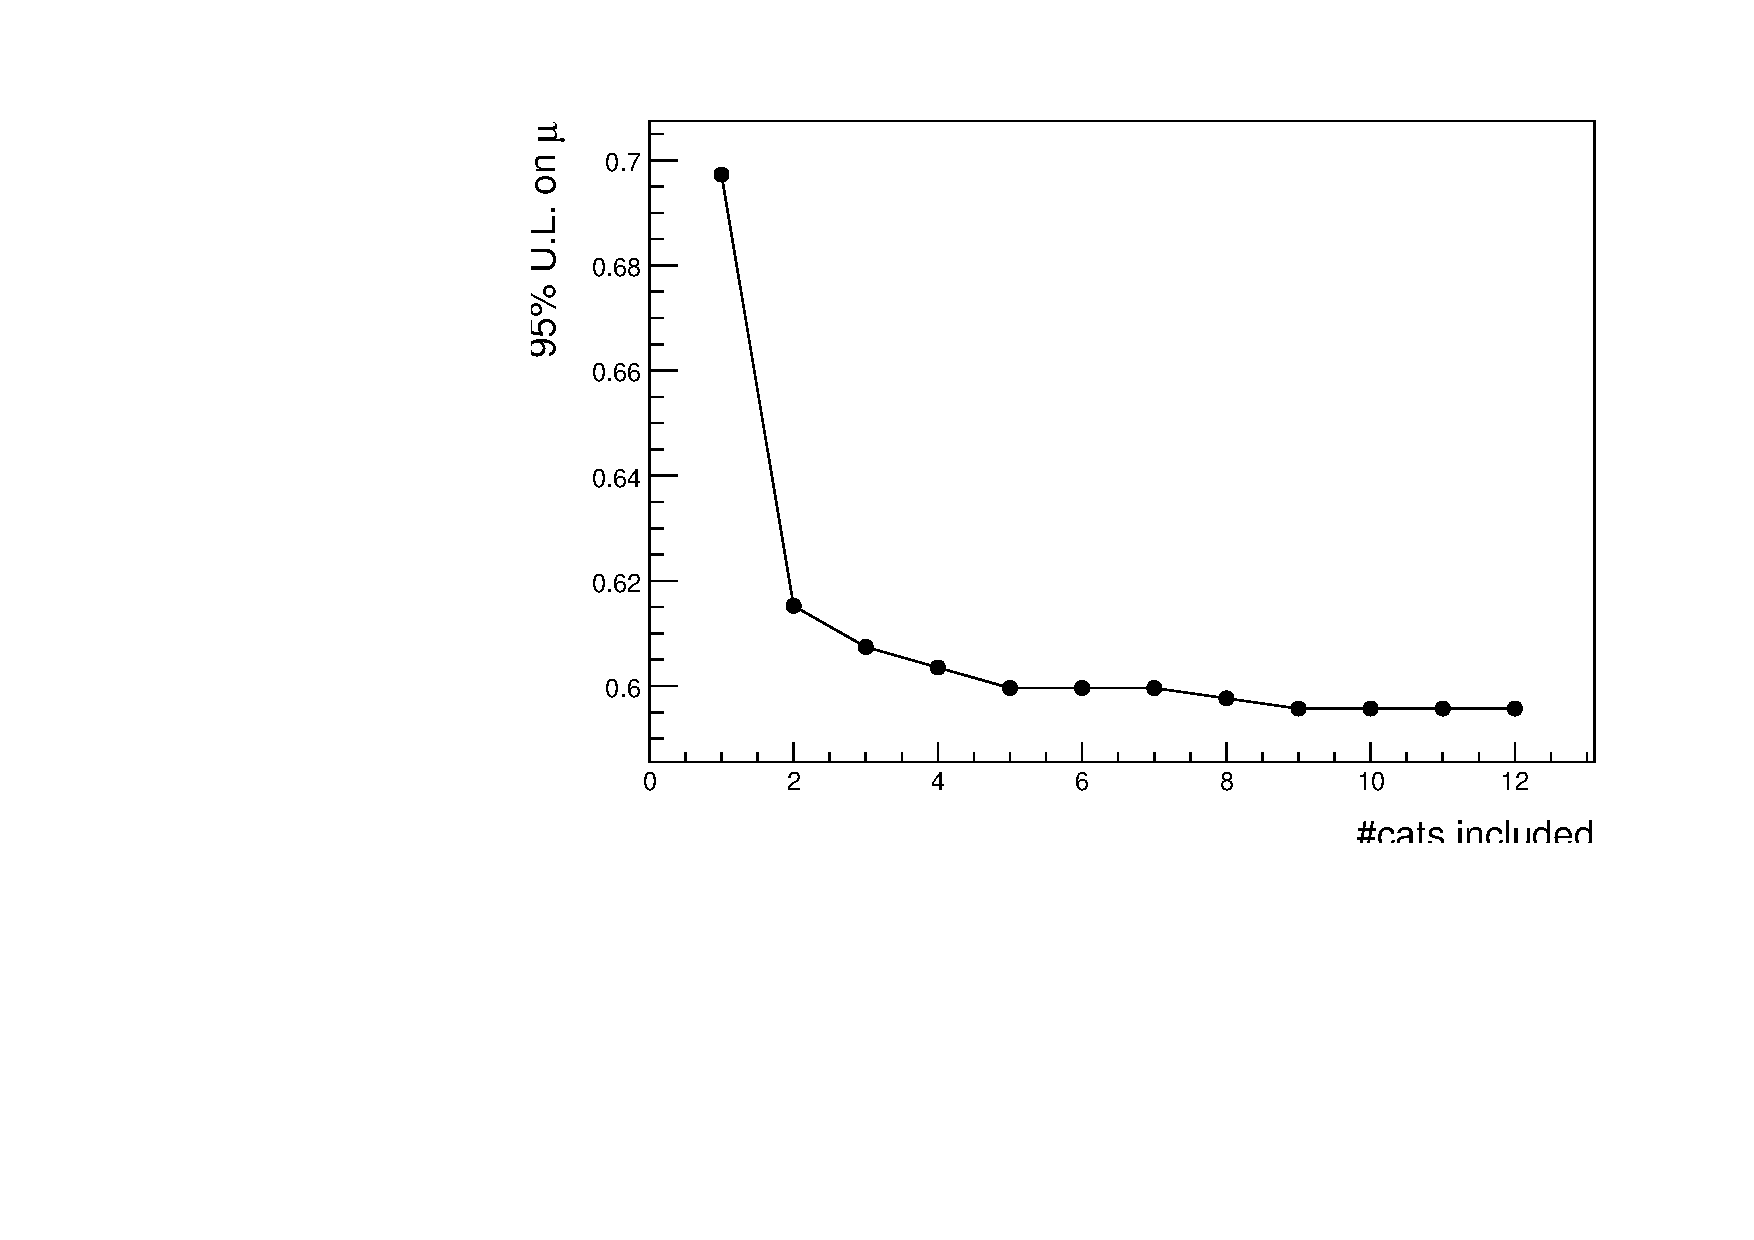
\includegraphics[width=0.31\textwidth]{figures/sensitivityStudy/MuVsCat_SMS_T1qqqq_2J_mGl1000_mLSP800.pdf}} \\
    \subfigure[{\scriptsize SMS\_T1qqqq\_2J\_mGl1400\_mLSP100}]{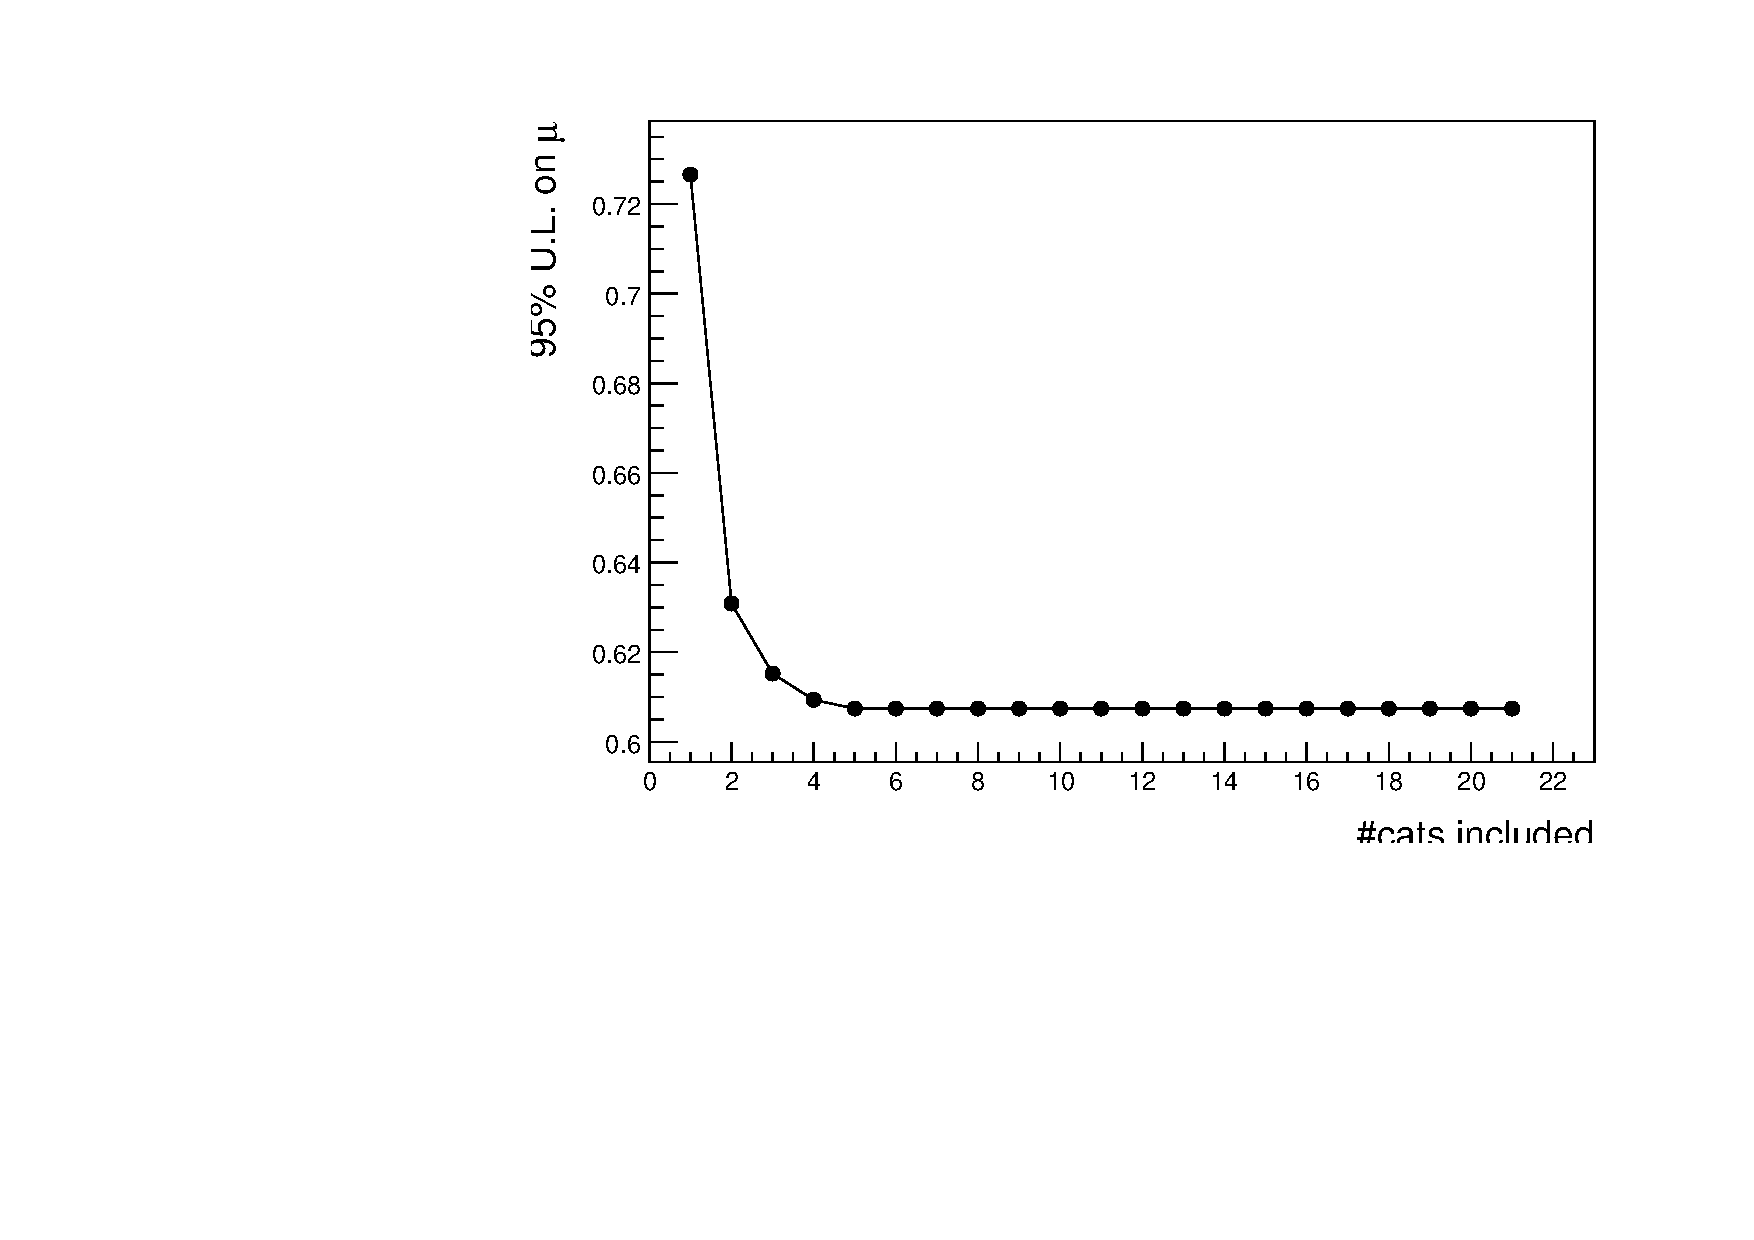
\includegraphics[width=0.31\textwidth]{figures/sensitivityStudy/MuVsCat_SMS_T1qqqq_2J_mGl1400_mLSP100.pdf}} ~~
    \subfigure[{\scriptsize SMS\_T1tttt\_2J\_mGl1200\_mLSP800}]{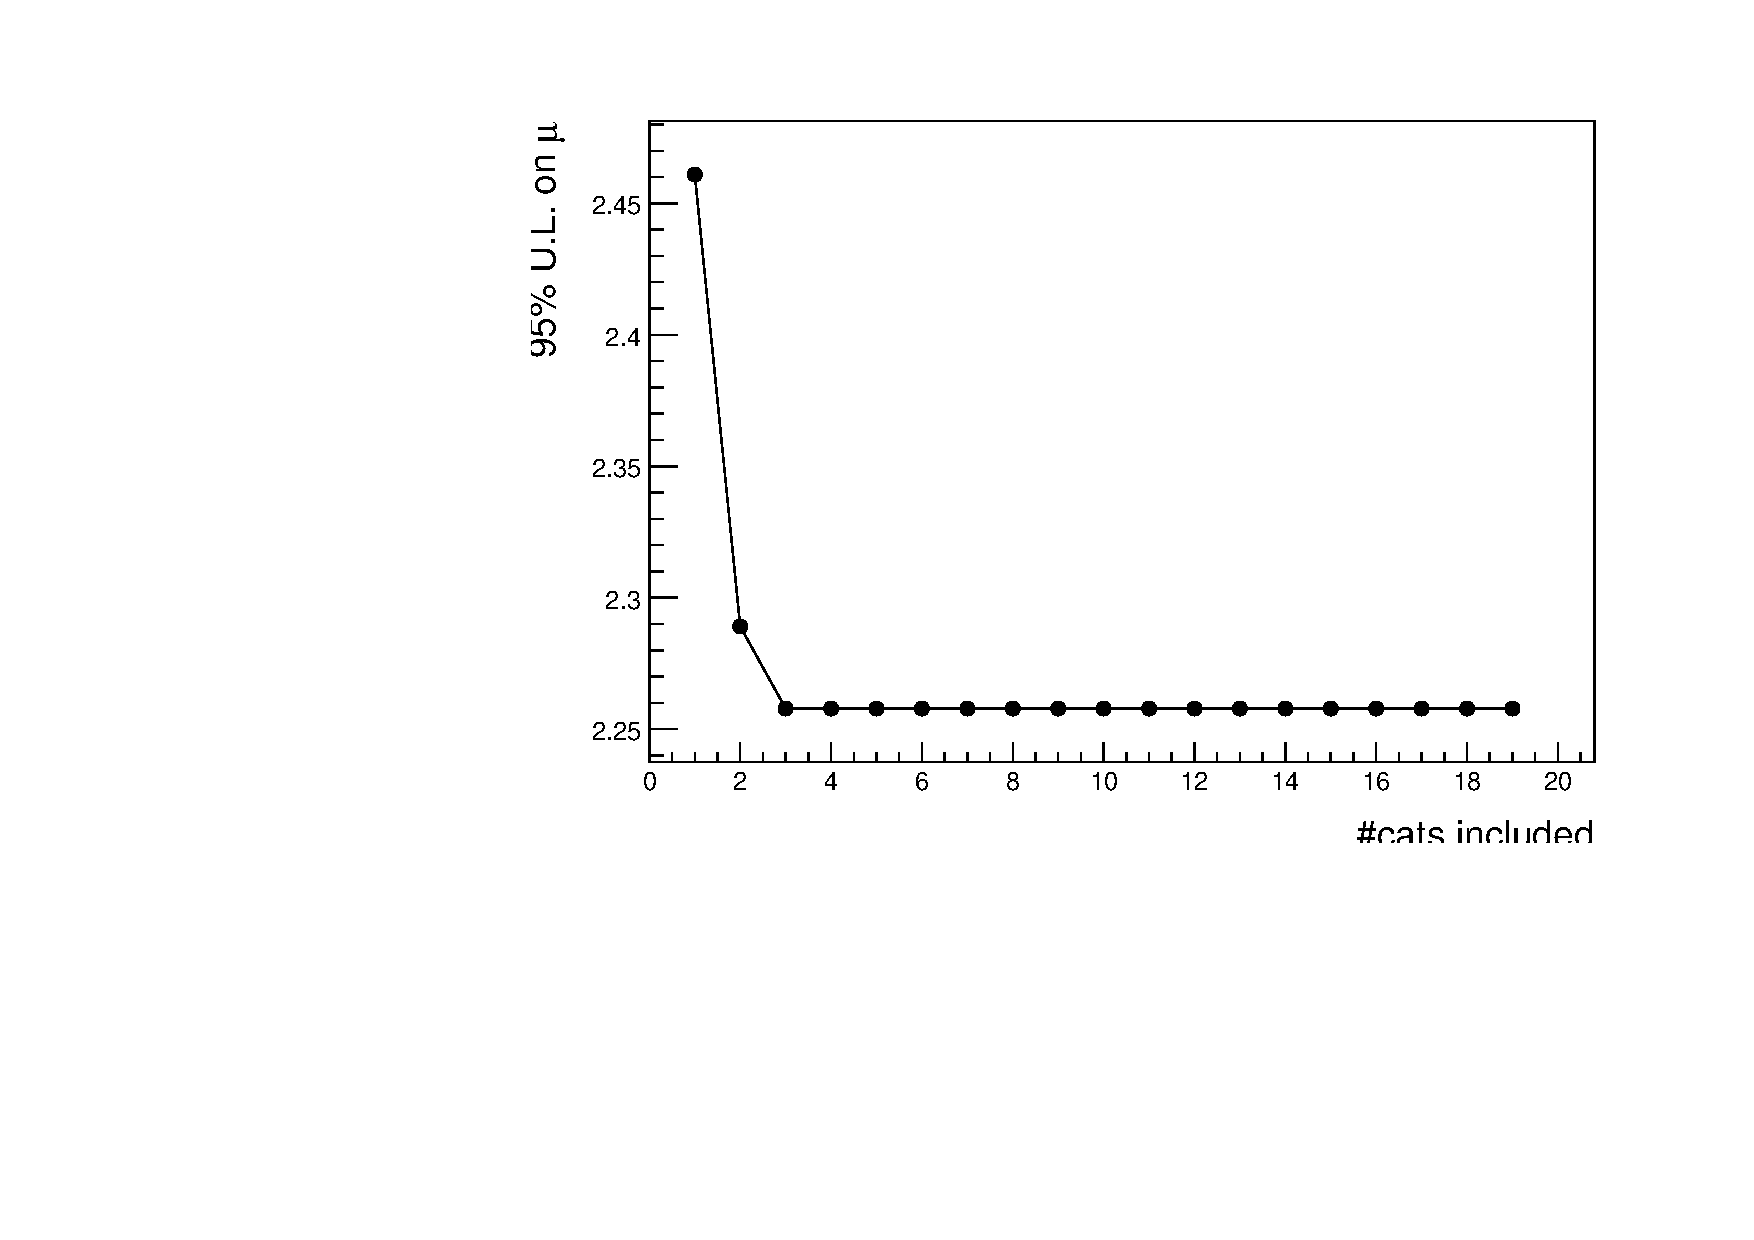
\includegraphics[width=0.31\textwidth]{figures/sensitivityStudy/MuVsCat_SMS_T1tttt_2J_mGl1200_mLSP800.pdf}} ~~
    \subfigure[{\scriptsize SMS\_T2bb\_2J\_mStop600\_mLSP580}]{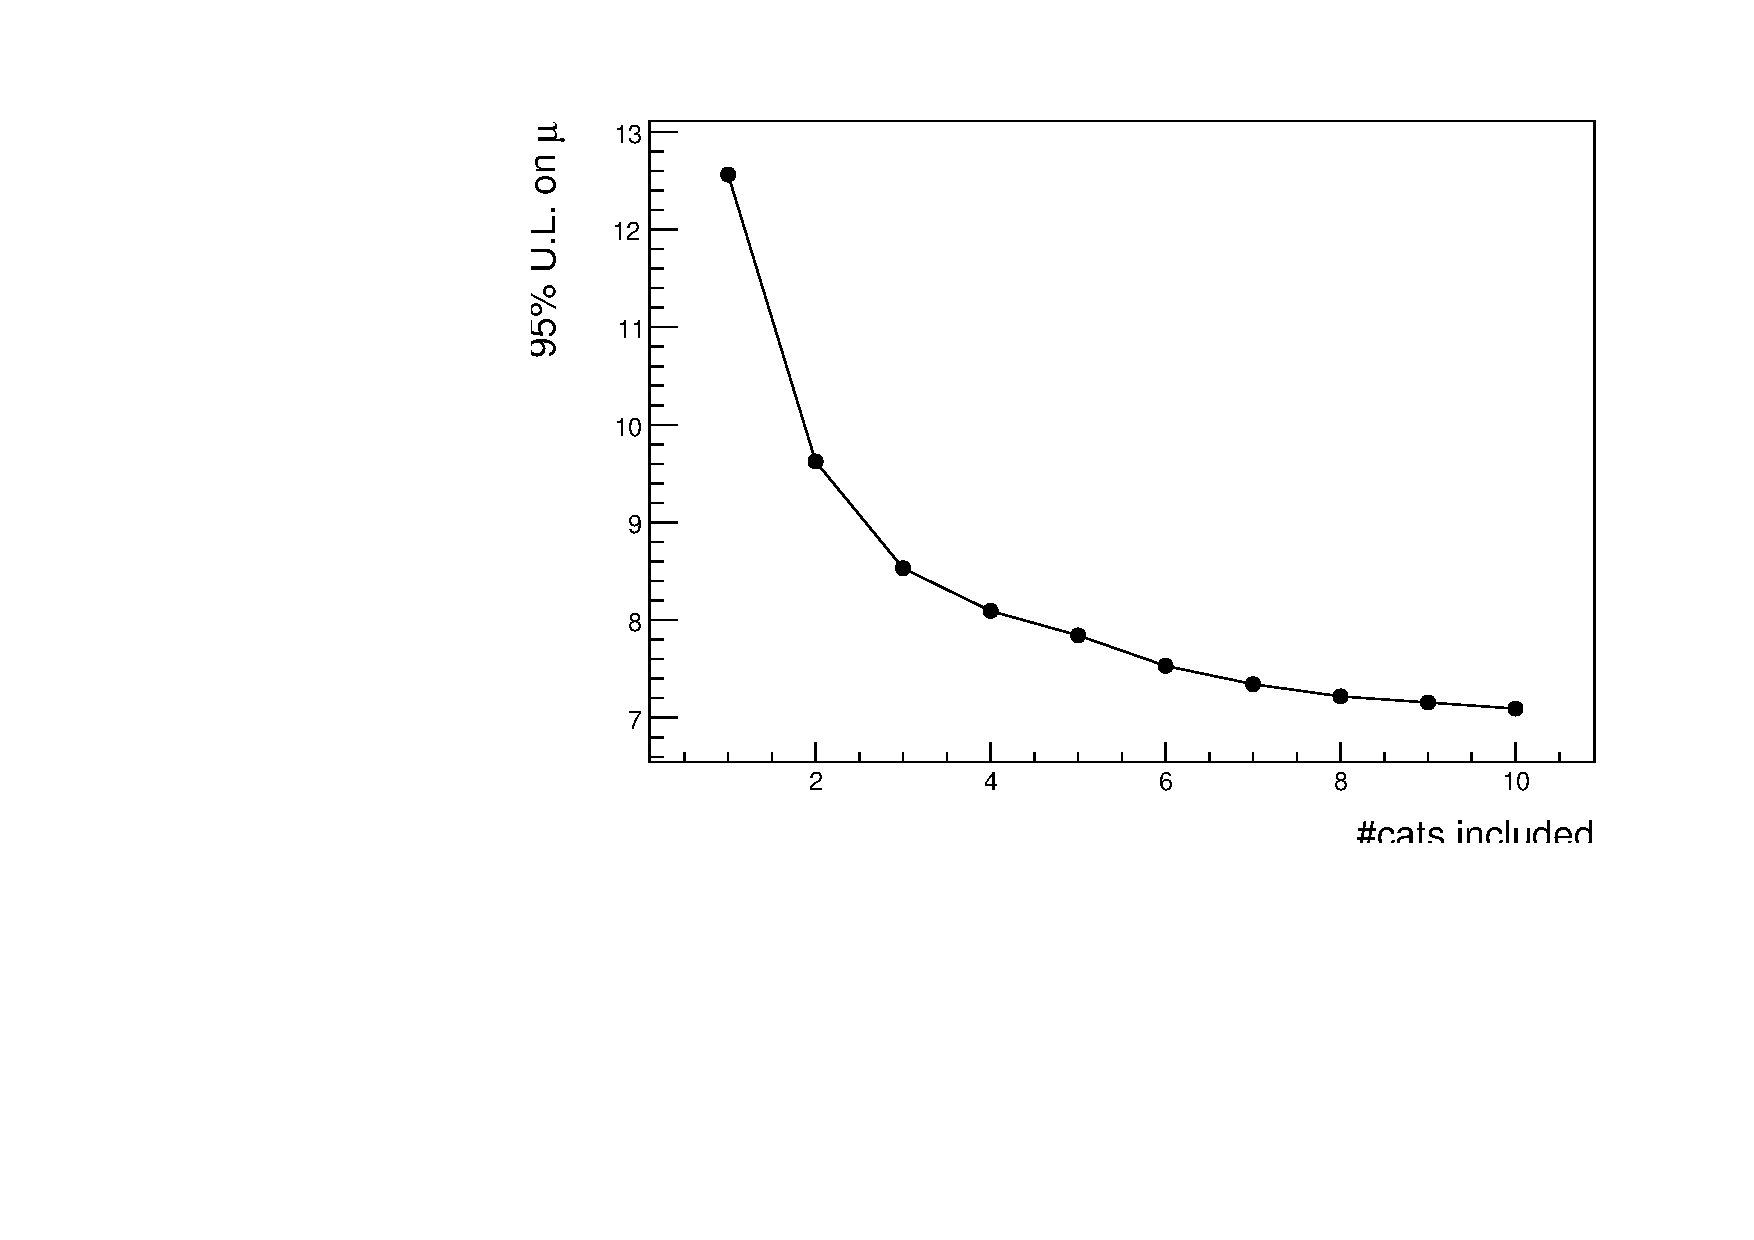
\includegraphics[width=0.31\textwidth]{figures/sensitivityStudy/MuVsCat_SMS_T2bb_2J_mStop600_mLSP580.pdf}} \\
    \subfigure[{\scriptsize SMS\_T2bb\_2J\_mStop900\_mLSP100}]{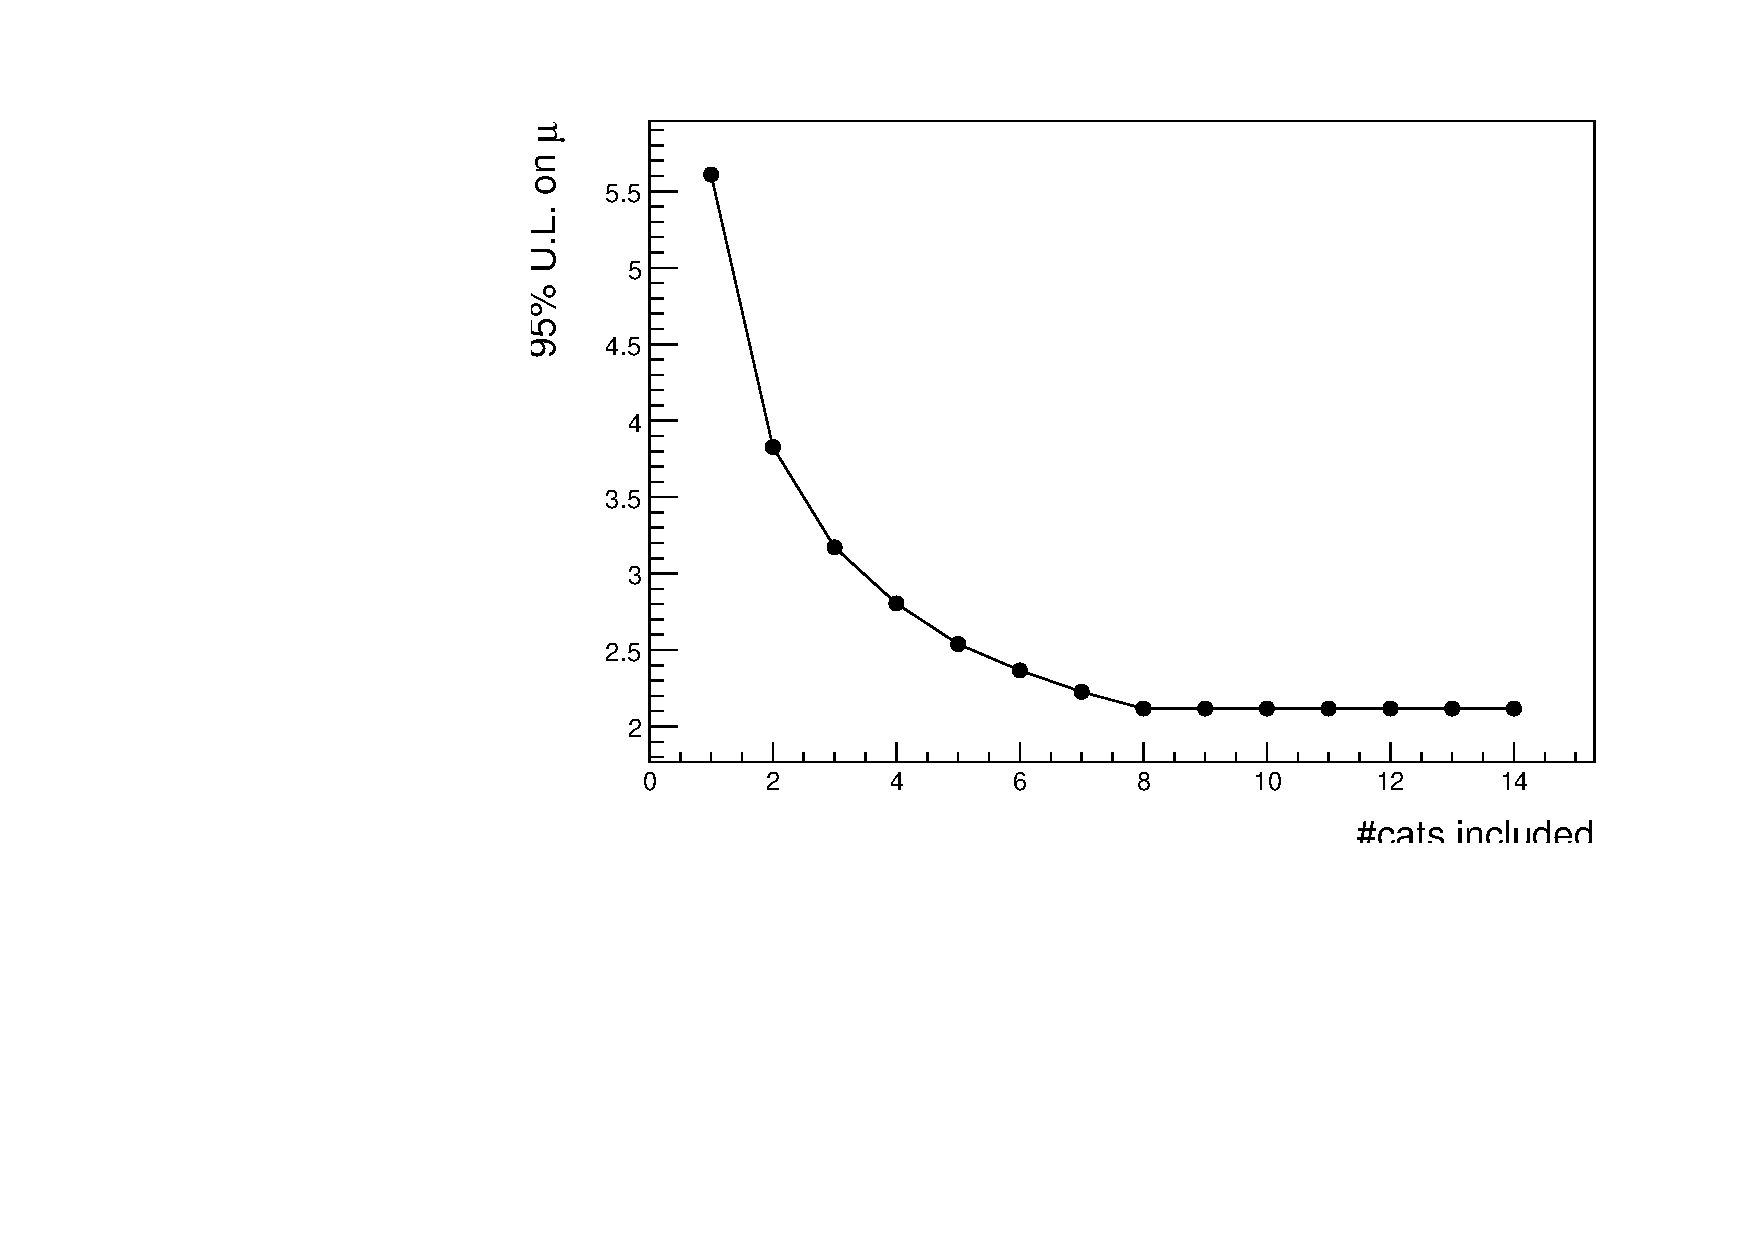
\includegraphics[width=0.31\textwidth]{figures/sensitivityStudy/MuVsCat_SMS_T2bb_2J_mStop900_mLSP100.pdf}} ~~
    \subfigure[{\scriptsize SMS\_T2qq\_2J\_mStop1200\_mLSP100}]{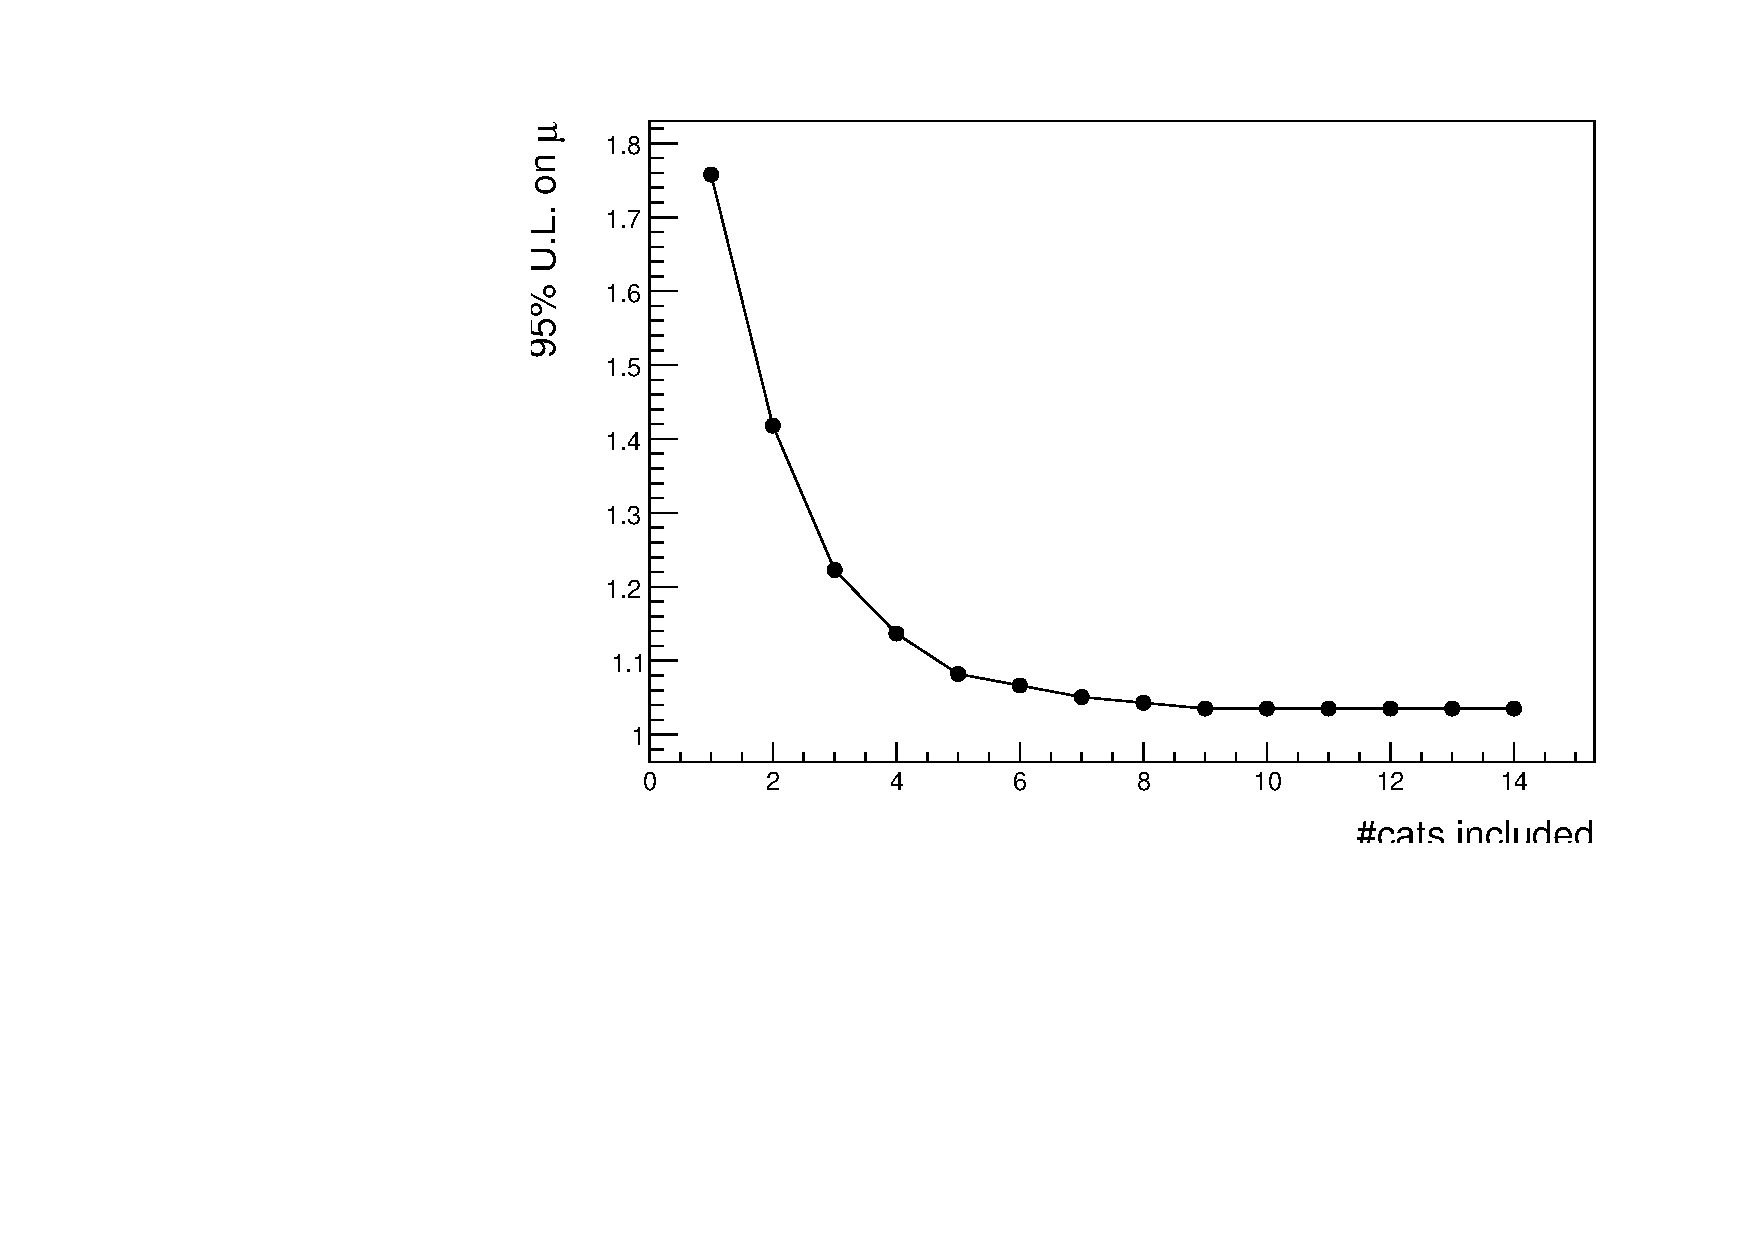
\includegraphics[width=0.31\textwidth]{figures/sensitivityStudy/MuVsCat_SMS_T2qq_2J_mStop1200_mLSP100.pdf}} ~~
    \subfigure[{\scriptsize SMS\_T2qq\_2J\_mStop600\_mLSP550}]{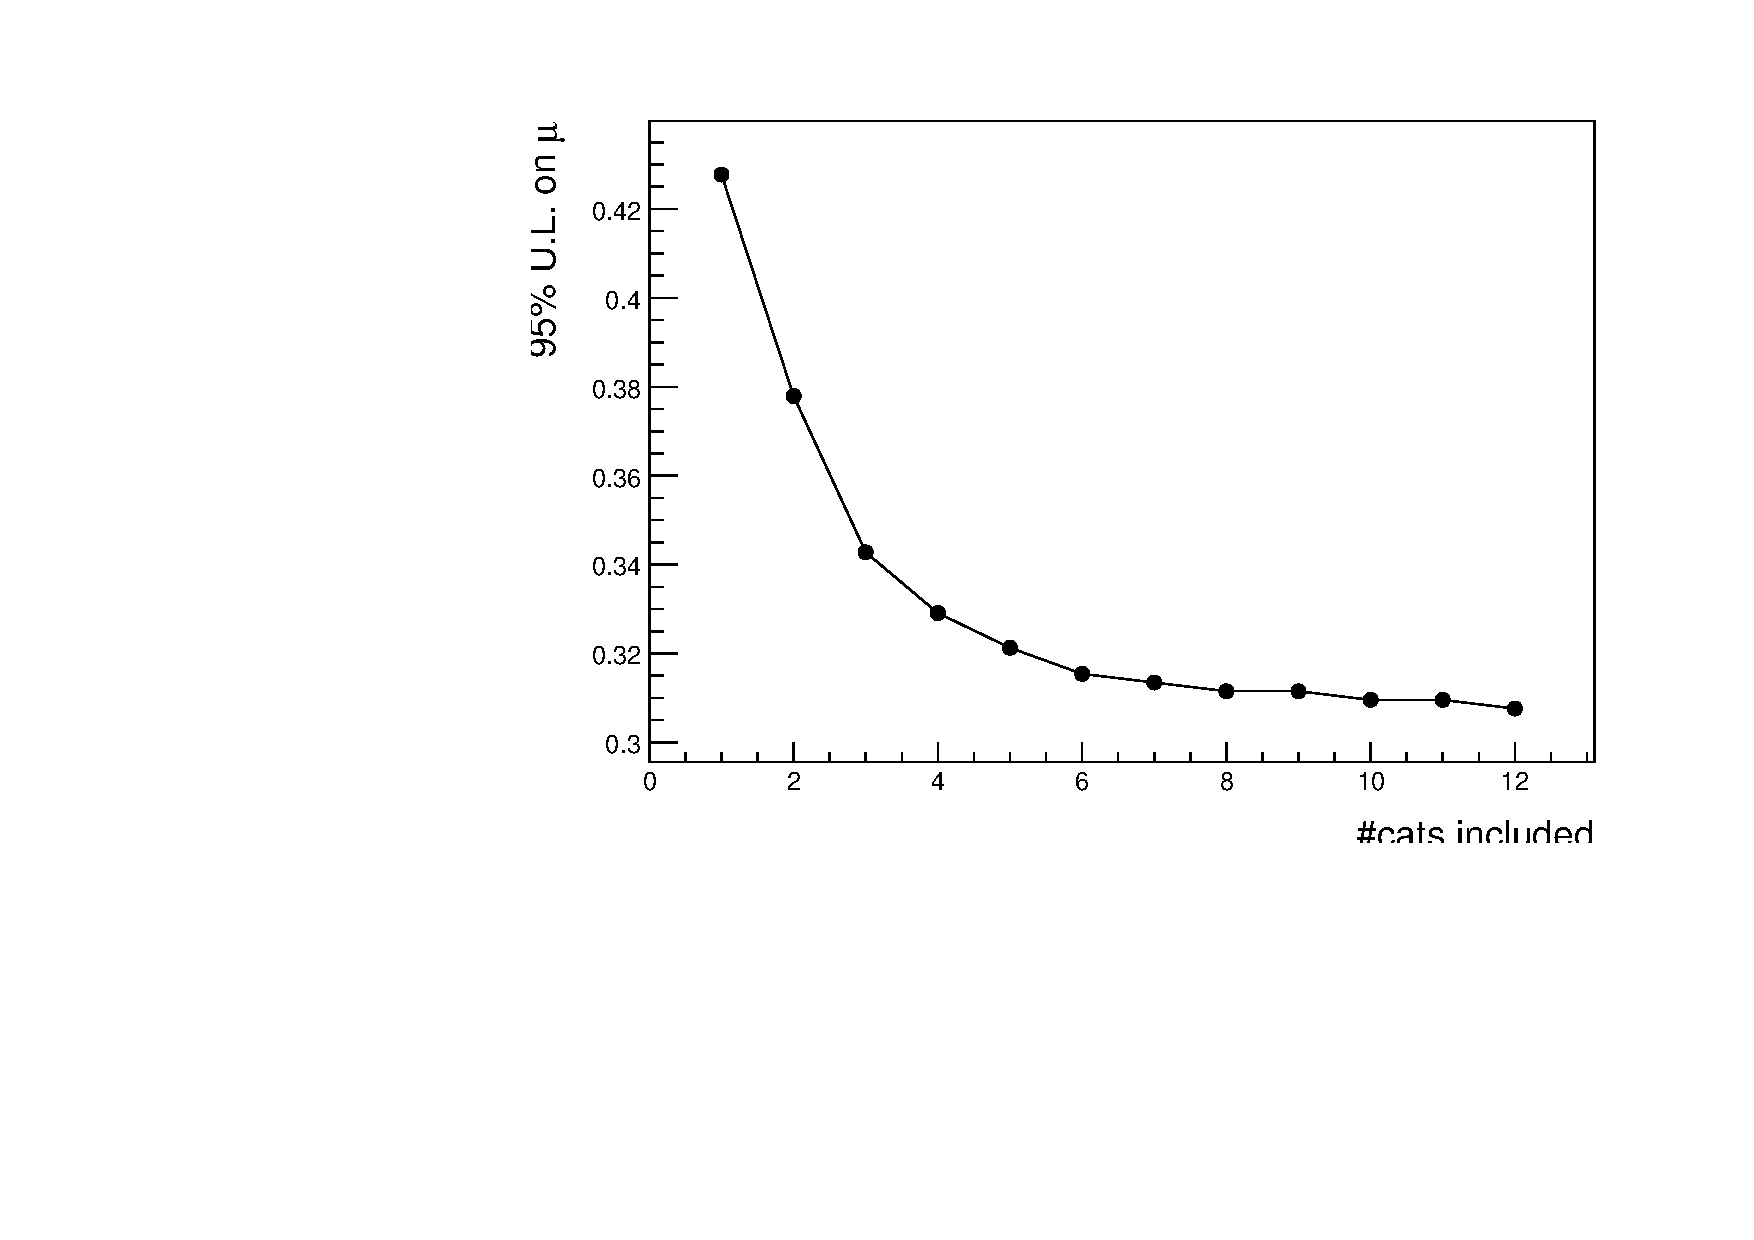
\includegraphics[width=0.31\textwidth]{figures/sensitivityStudy/MuVsCat_SMS_T2qq_2J_mStop600_mLSP550.pdf}} \\
    \subfigure[{\scriptsize SMS\_T2tt\_2J\_mStop425\_mLSP325}]{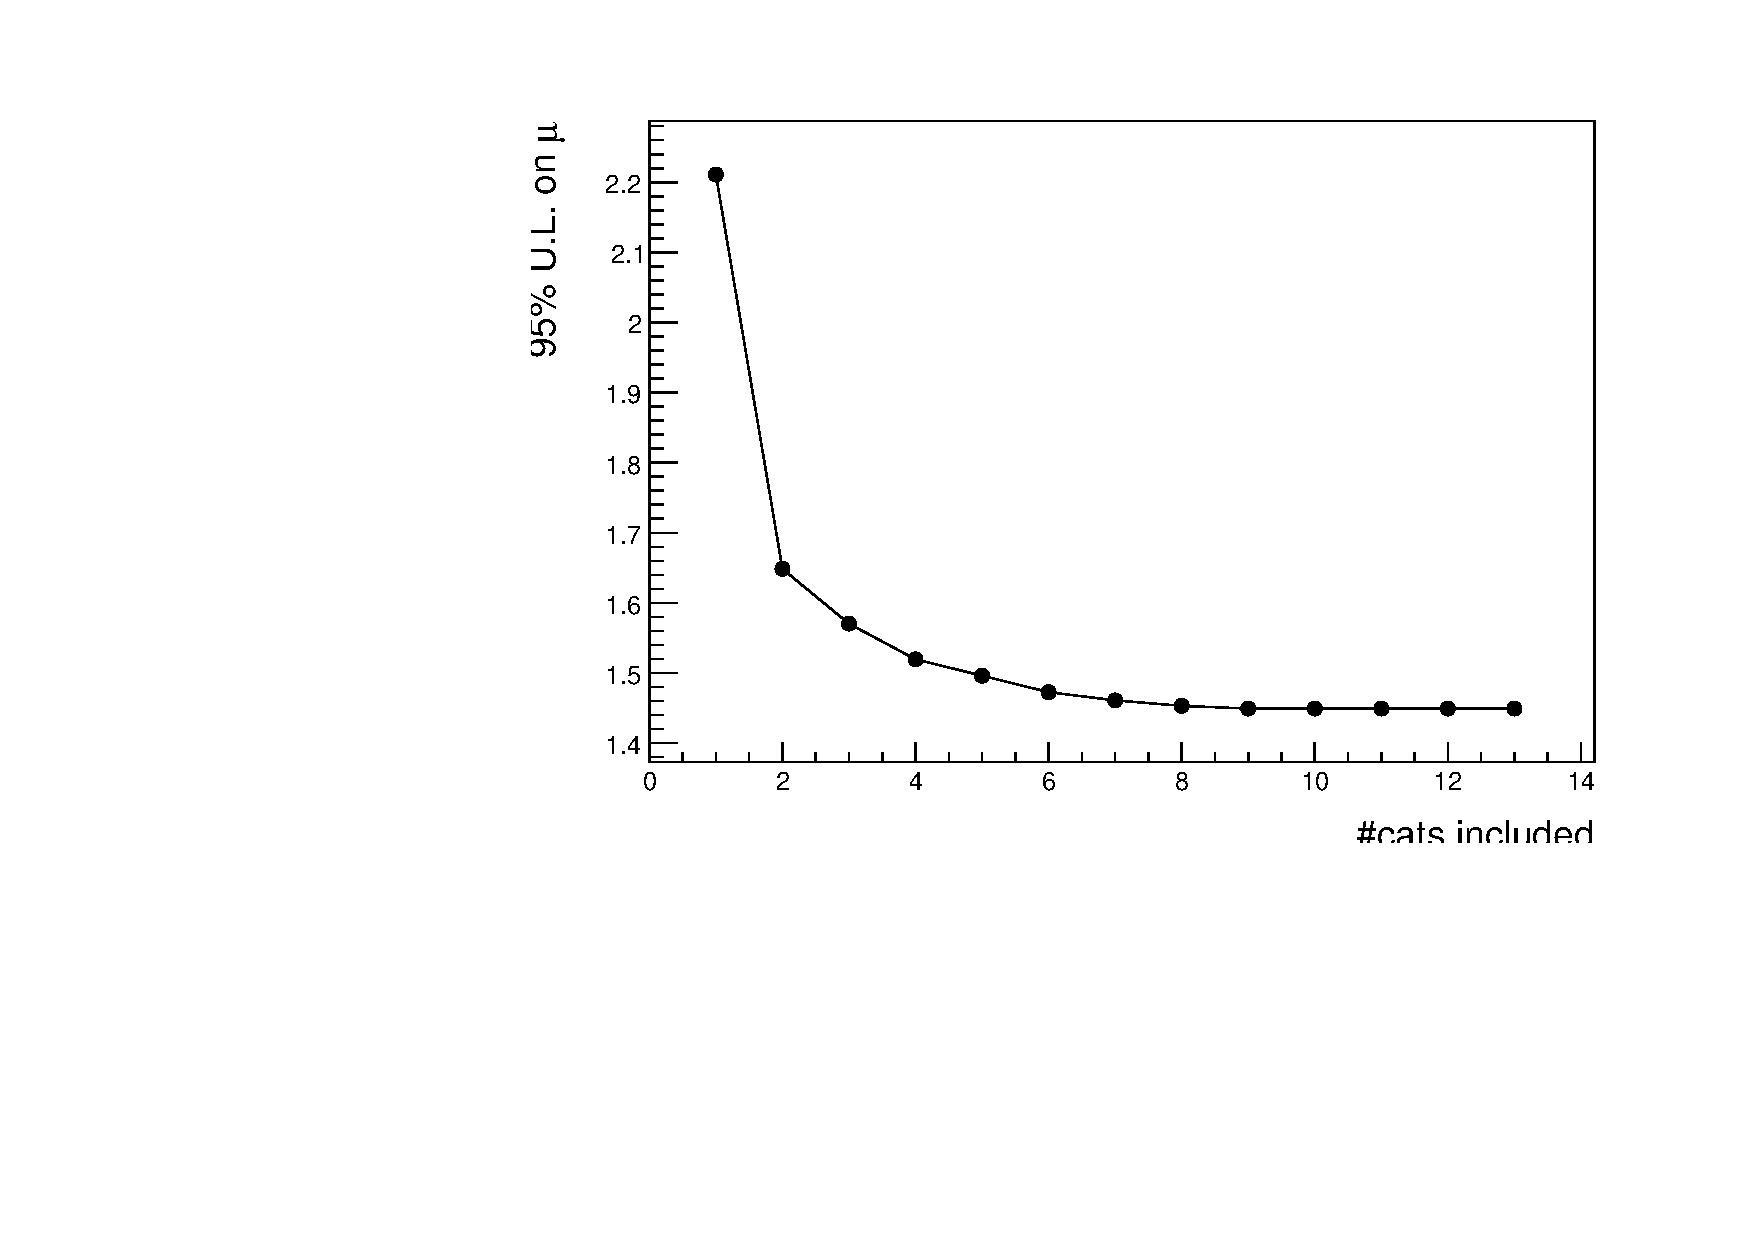
\includegraphics[width=0.31\textwidth]{figures/sensitivityStudy/MuVsCat_SMS_T2tt_2J_mStop425_mLSP325.pdf}} ~~
    \subfigure[{\scriptsize SMS\_T2tt\_2J\_mStop500\_mLSP325}]{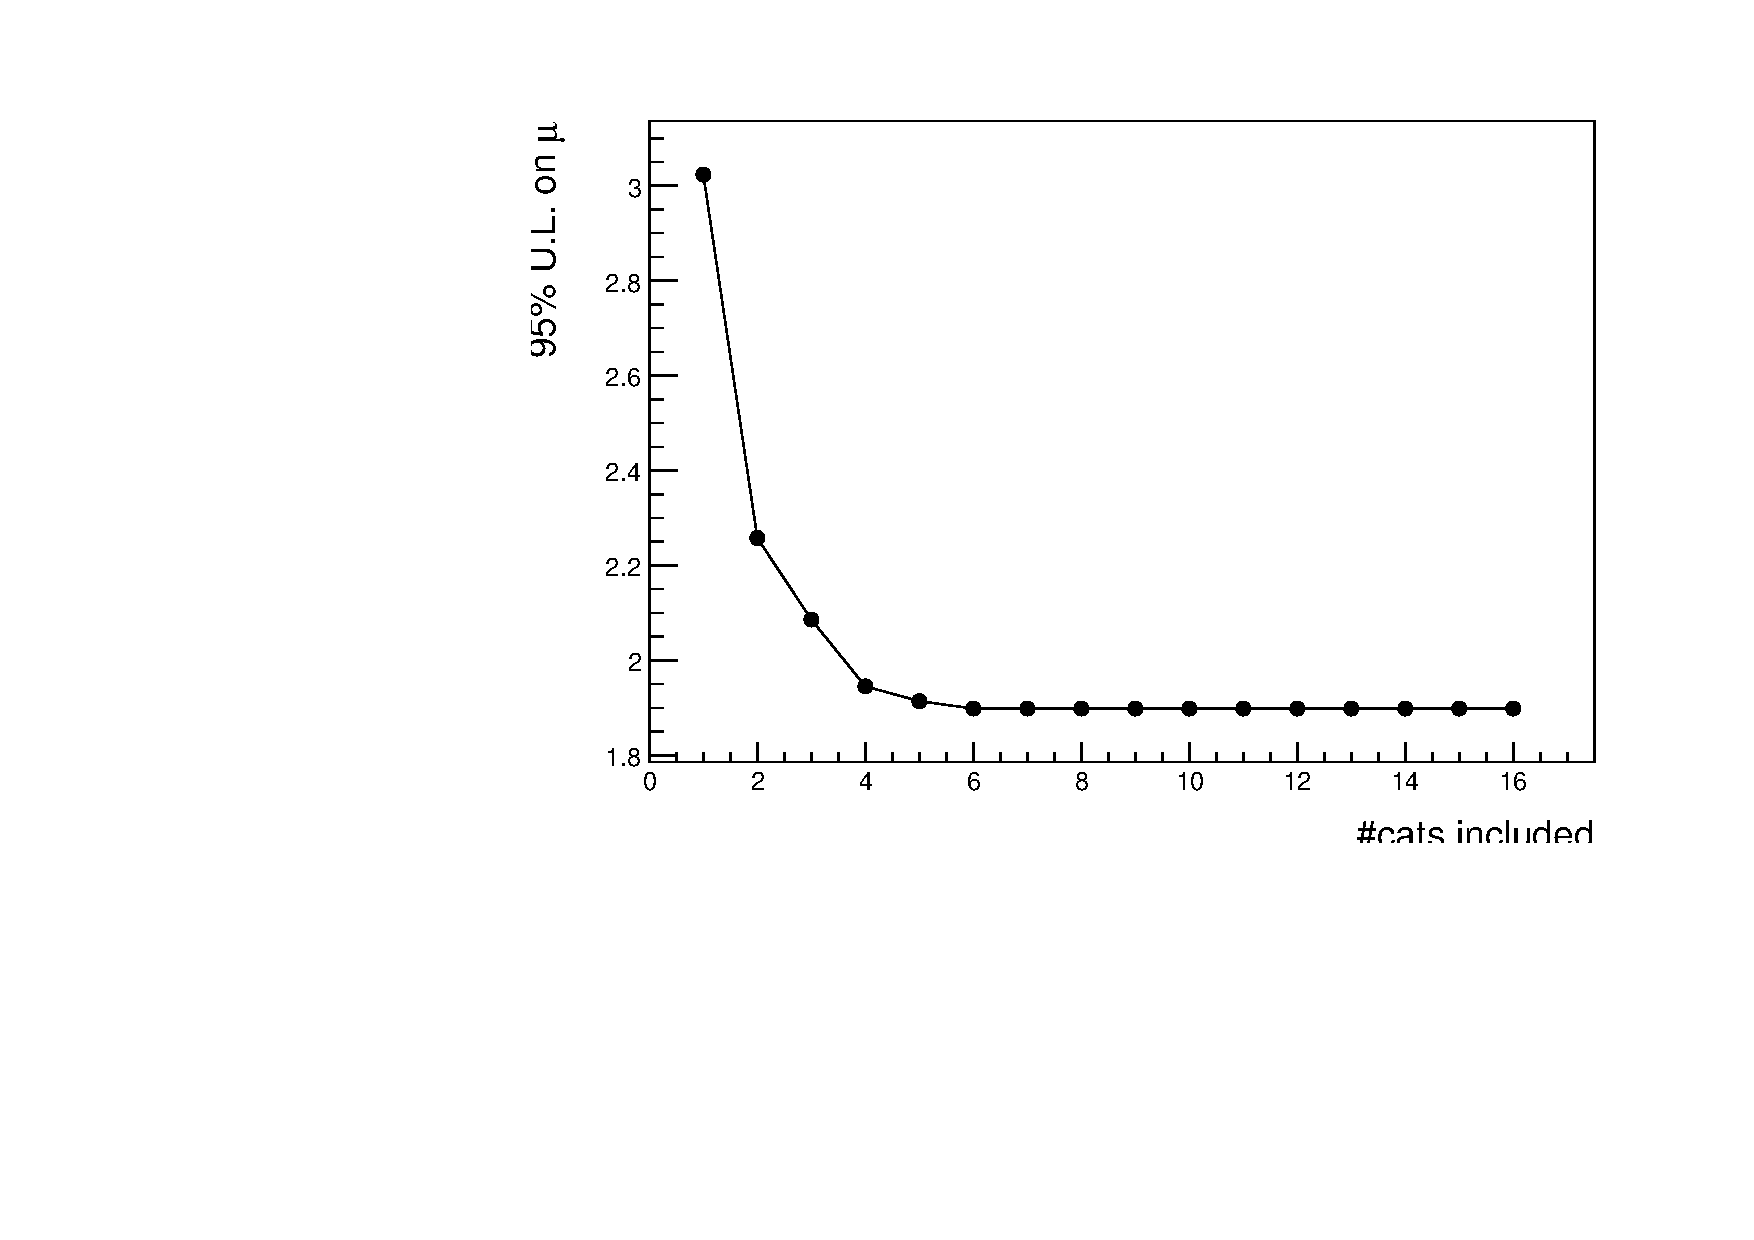
\includegraphics[width=0.31\textwidth]{figures/sensitivityStudy/MuVsCat_SMS_T2tt_2J_mStop500_mLSP325.pdf}} ~~
    \subfigure[{\scriptsize SMS\_T2tt\_2J\_mStop650\_mLSP325}]{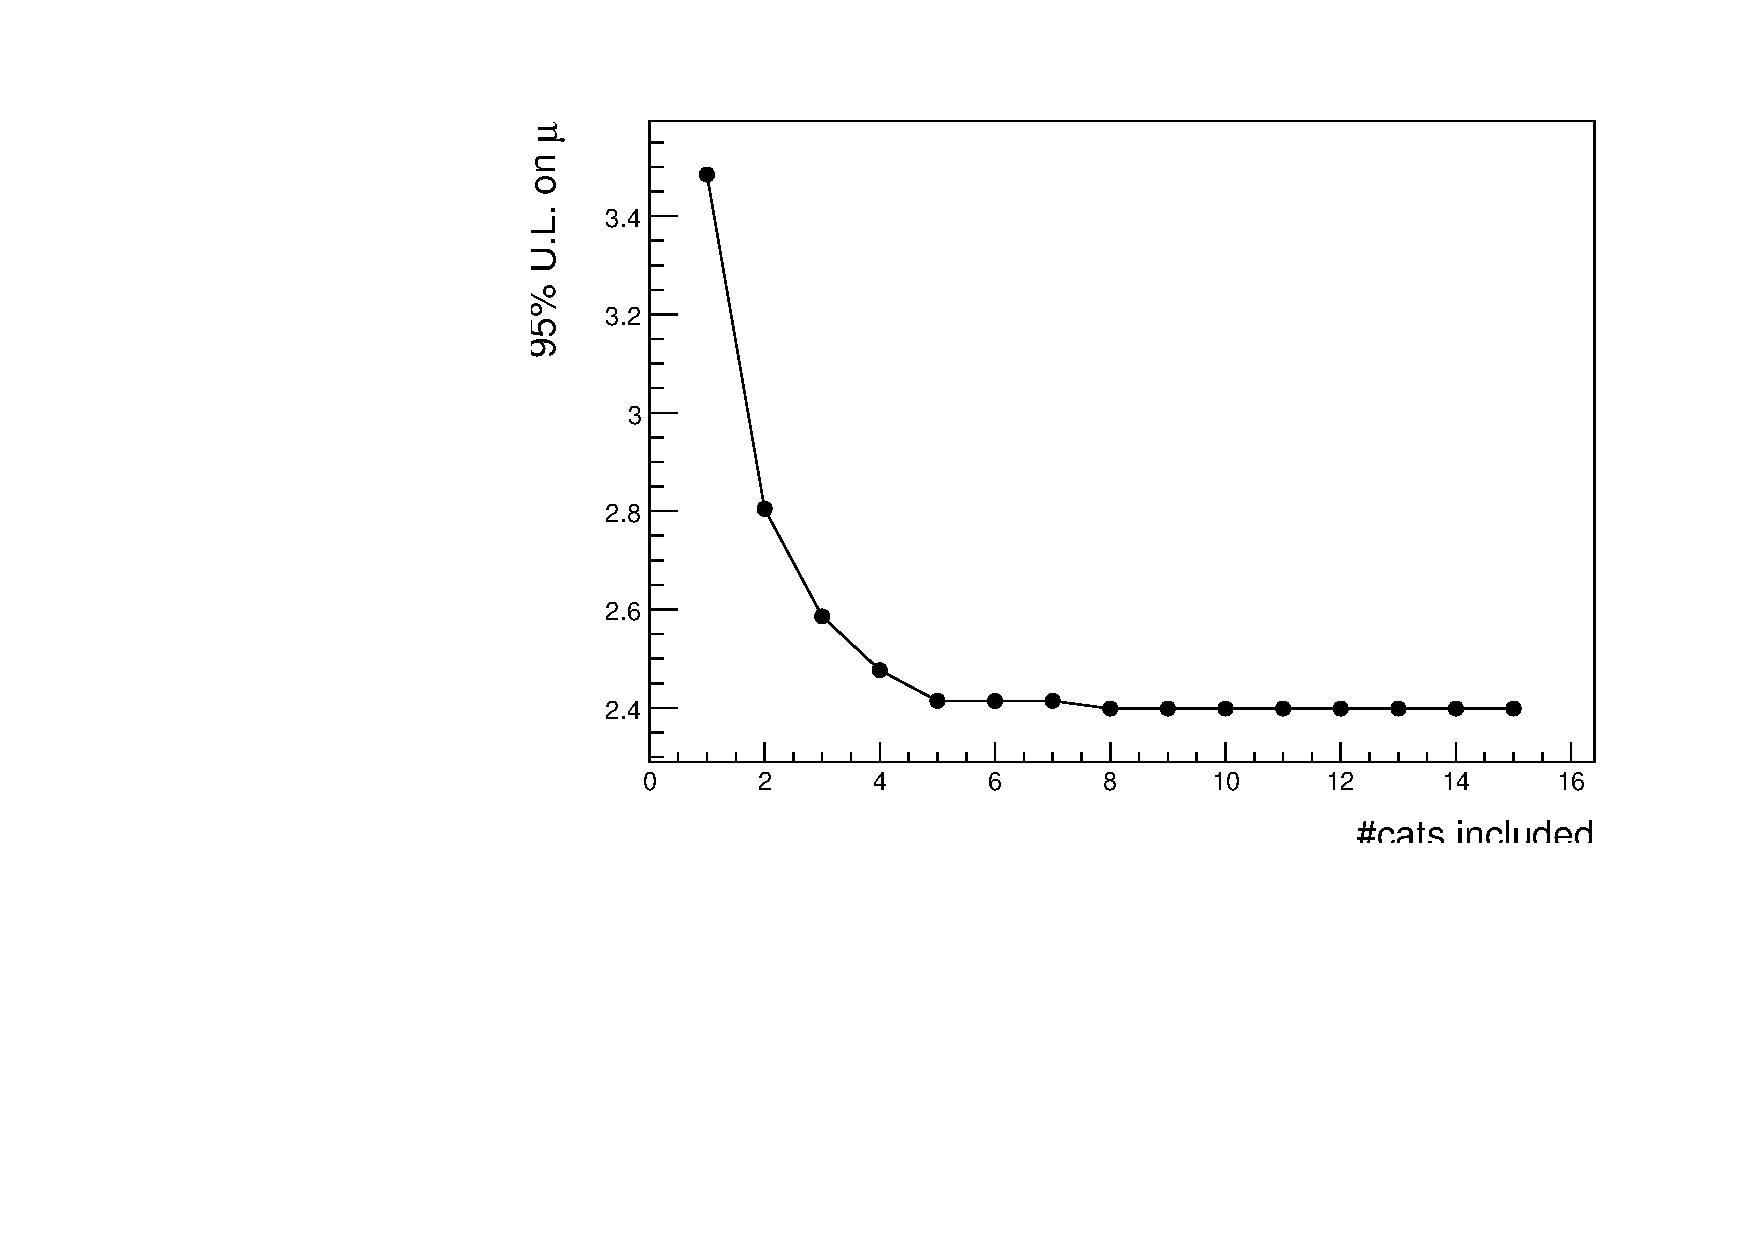
\includegraphics[width=0.31\textwidth]{figures/sensitivityStudy/MuVsCat_SMS_T2tt_2J_mStop650_mLSP325.pdf}} \\
    \subfigure[{\scriptsize SMS\_T2tt\_2J\_mStop850\_mLSP100}]{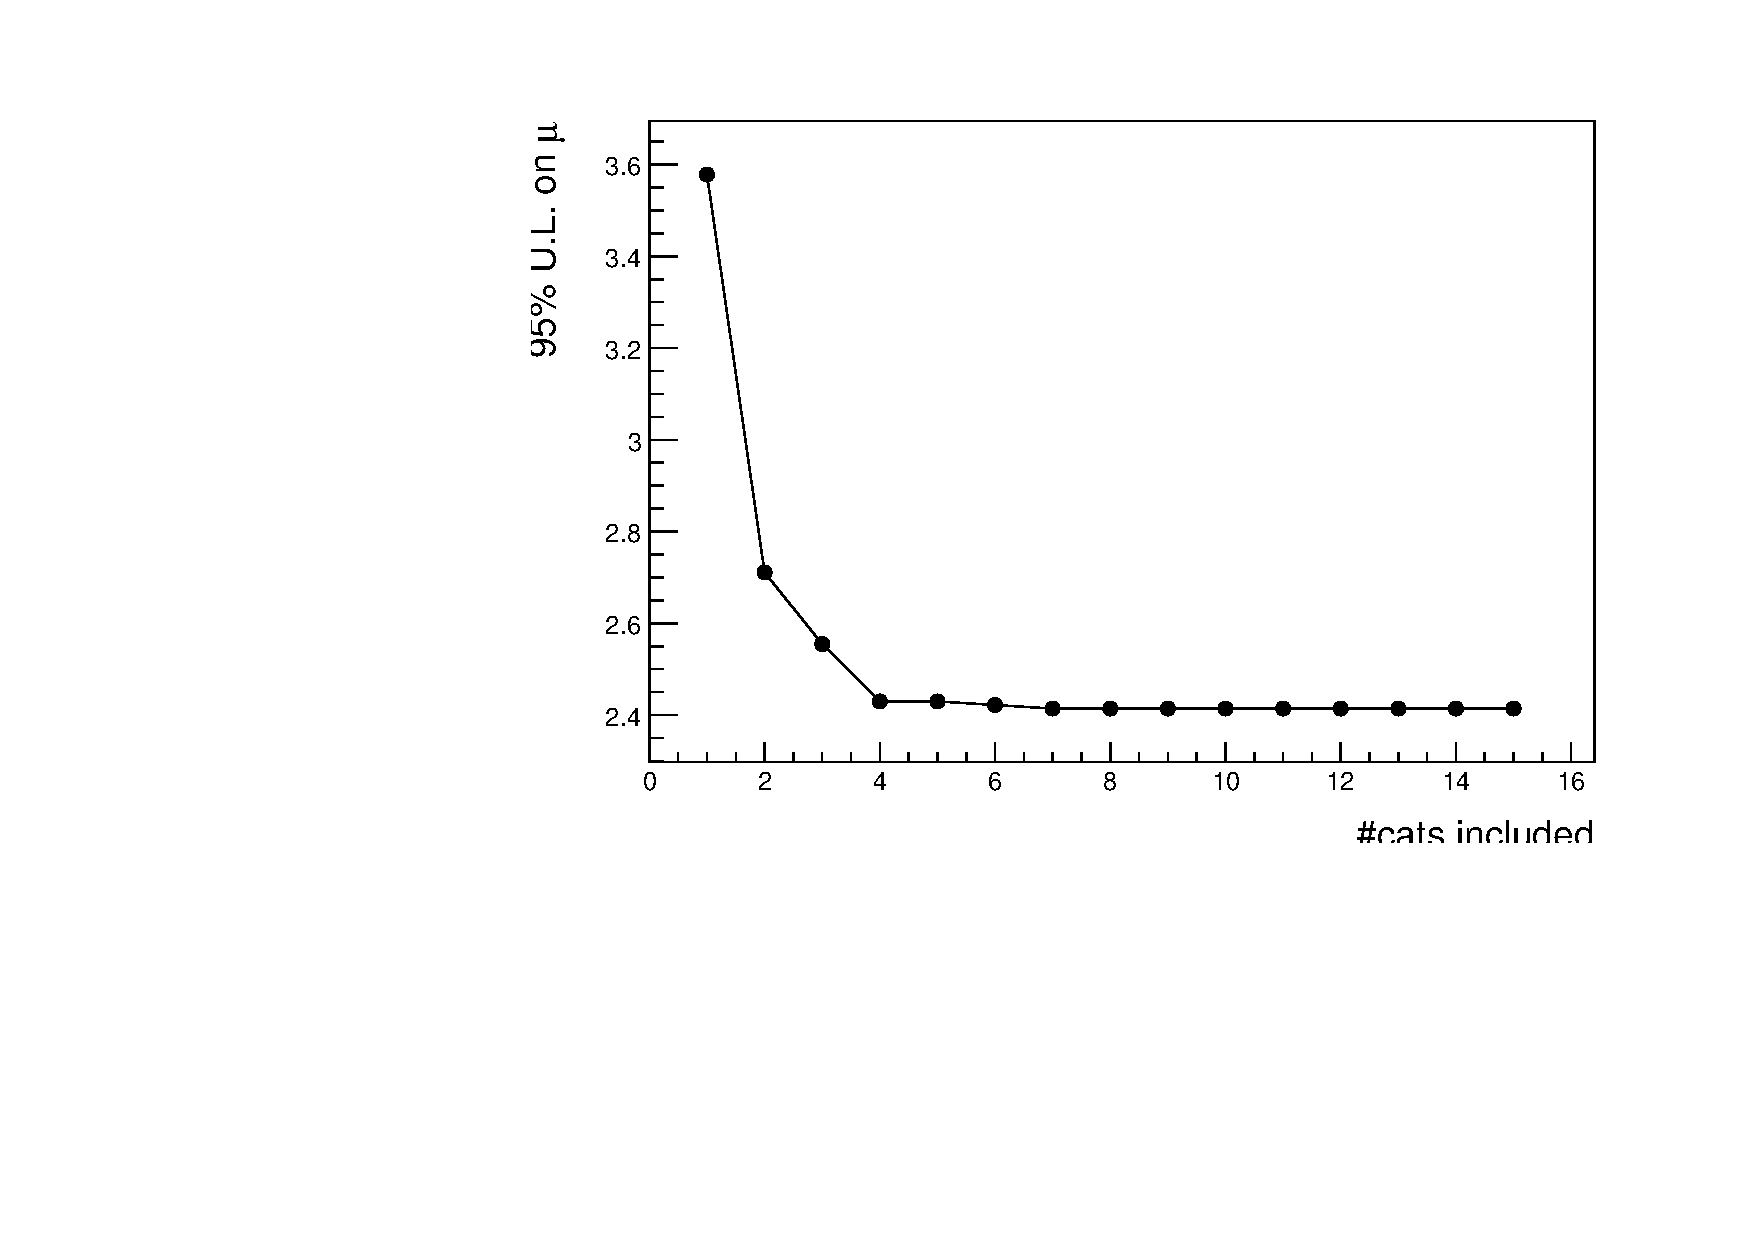
\includegraphics[width=0.31\textwidth]{figures/sensitivityStudy/MuVsCat_SMS_T2tt_2J_mStop850_mLSP100.pdf}}
    \caption{Upper limits on the signal strength as a function of the number of $(\njet,\nb)$ categories included in the fit.}
    \label{fig:muVsCat}
  \end{center}
\end{figure}



%%____________________________________________________________________________||
